% For SVG
\documentclass[dvisvgm]{minimal}



\usepackage{tikz}
\usetikzlibrary{trees, calc}


\begin{document}
\tikzset{
    every node/.style={
    draw=black,
    anchor=west,
    }
}
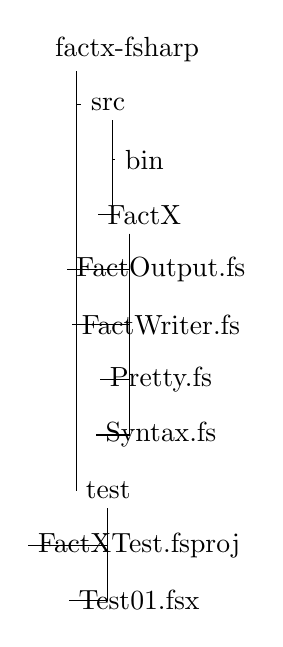
\begin{tikzpicture}[
    grow via three points={
        one child at (0.8, -0.7) and two children at (0.8, -0.7) and (0.8, -1.4)
    },
    edge from parent path = {
        ($(\tikzparentnode\tikzparentanchor)+(.4cm,0pt)$) |- (\tikzchildnode\tikzchildanchor)
    },
    growth parent anchor=west,
    parent anchor=south west,
    ]
    \node {factx-fsharp}
        child {node {src}
            child {node {bin}}
            child {node {FactX}
                child {node {FactOutput.fs}}
                child {node {FactWriter.fs}}
                child {node {Pretty.fs}}
                child {node {Syntax.fs}}
            }
        }
        child [missing] {}
        child [missing] {}
        child [missing] {}  
        child [missing] {}
        child [missing] {}
        child [missing] {} 
        child {node {test}
            child {node {FactXTest.fsproj}}
            child {node {Test01.fsx}}
        };
\end{tikzpicture}
\end{document}
